\chapter{Cài đặt và thử nghiệm}
\label{ch:caidat}

\begin{muctieu}
Chương này trình bày môi trường phát triển, cách tích hợp các thành phần, giao diện và trạng thái kiểm tra phần mềm.
\end{muctieu}

\section{Môi trường triển khai}
Dự án gồm frontend React/Vite và backend FastAPI. Docker Compose cấu hình frontend tại cổng 5173, backend tại cổng 8000, SQLite trong backend và thư mục uploads để lưu tệp. Có thể truy cập giao diện bằng \url{http://localhost:5173} và tài liệu API bằng \url{http://localhost:8000/docs}. Địa chỉ \code{0.0.0.0} dùng để dịch vụ lắng nghe kết nối bên trong môi trường chạy, không phải URL người dùng nhập vào trình duyệt.

Bộ đọc OCR phụ thuộc Tesseract và dữ liệu ngôn ngữ. Trong cấu hình Docker dự án, các thành phần OCR được cài trong image backend; khi chạy trực tiếp trên Windows, cần cài Tesseract cùng dữ liệu Anh/Việt theo README. Phiên bản phần mềm và cấu hình máy dùng để chạy lần cuối cần được bổ sung trước khi nộp.

\section{Các thành phần chính}
Frontend gọi API theo các miền chức năng và hiển thị trạng thái tải, lỗi hoặc kết quả. Backend dùng các router riêng để xử lý xác thực, vị trí, ứng viên/CV, matching, dashboard và model. Bộ phân tích CV tạo văn bản trích xuất và dữ liệu ứng viên; MatchingEngine tính các điểm tiêu chí và trả về giải thích cùng các kỹ năng đã khớp/thiếu. Pipeline Random Forest là một nhánh dự đoán riêng; API có thể trả chế độ fallback khi artifact mô hình chưa được nạp.

\section{Giao diện và demo}
Hình~\ref{fig:cvreview} là ảnh giao diện xem lại một CV minh họa, dùng để quan sát cấu trúc thông tin sau phân tích. Nội dung hồ sơ trong ảnh là dữ liệu mẫu, không phải hồ sơ người dùng thật.

\begin{figure}[H]
\centering
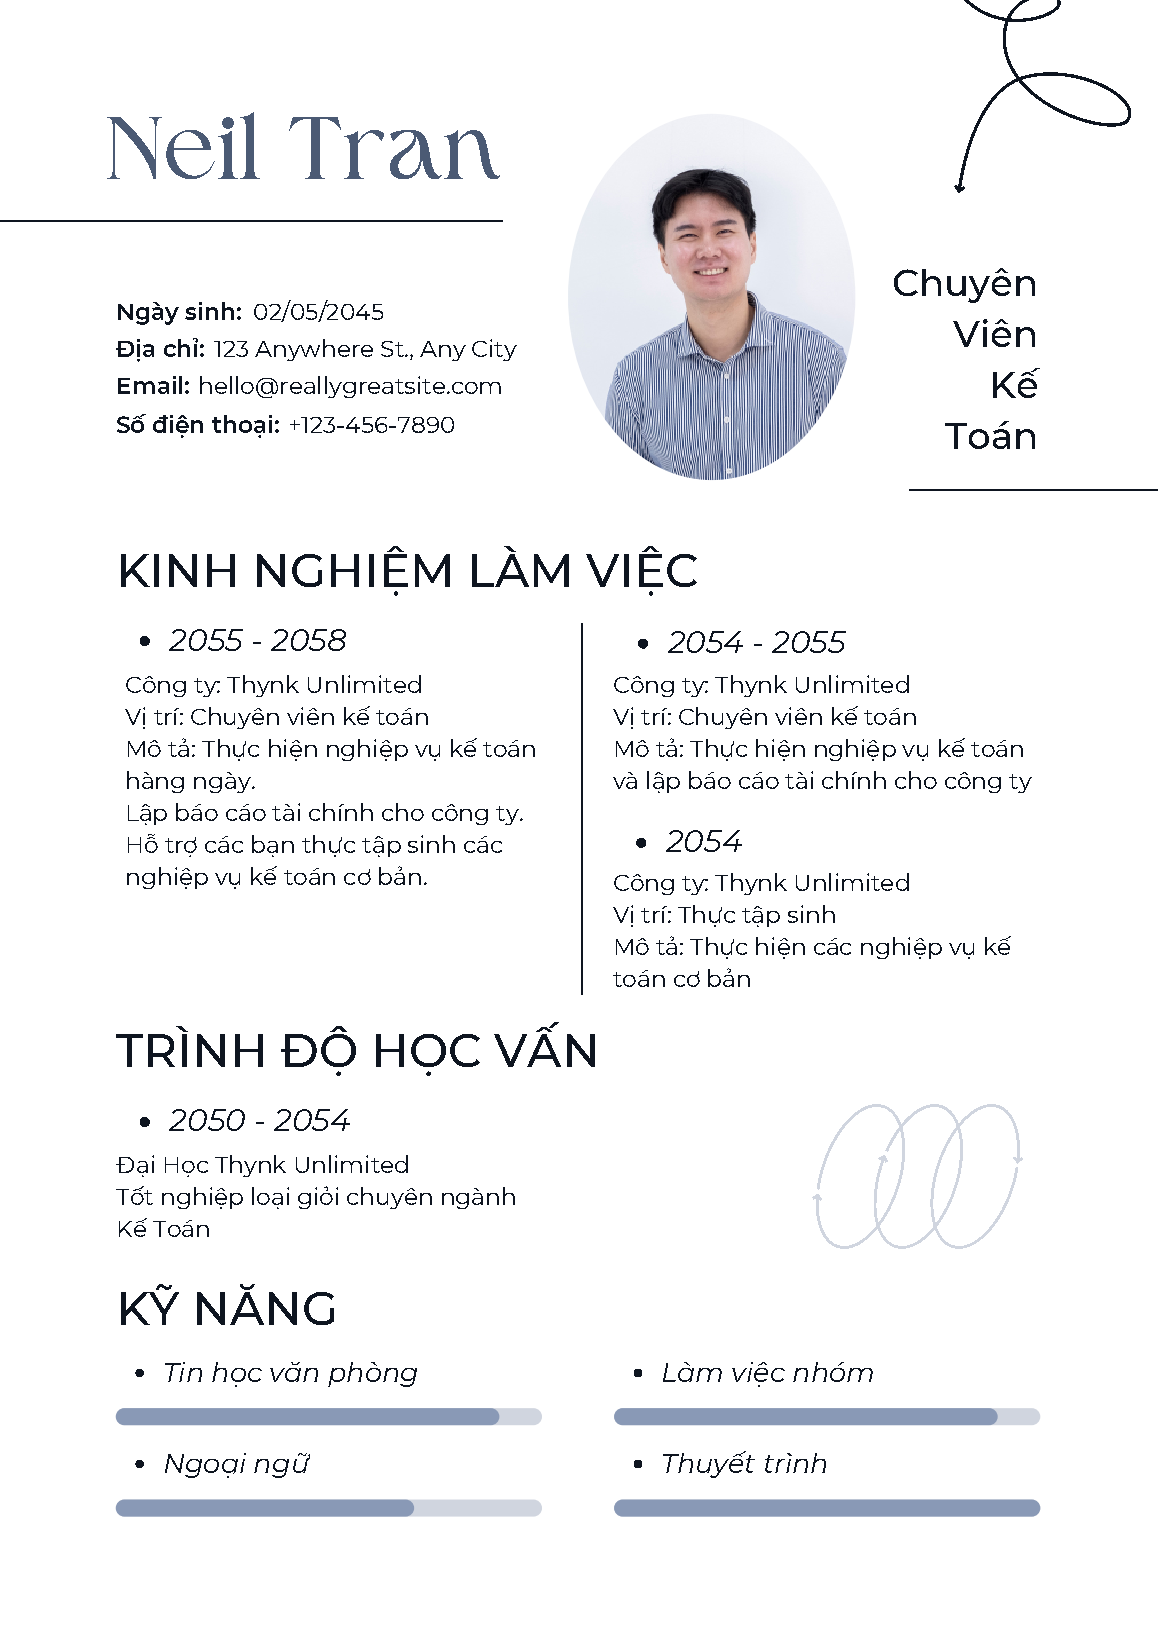
\includegraphics[width=0.66\textwidth]{hinh/cv-review.png}
\caption{Giao diện xem lại hồ sơ CV minh họa sau khi trích xuất.}
\label{fig:cvreview}
\end{figure}

\section{Kiểm thử}
Kho mã có các bộ kiểm tra cho bộ phân tích CV, thành phần cốt lõi, pipeline huấn luyện và dịch vụ embedding. Báo cáo này chưa ghi nhận một lần chạy kiểm thử cuối trên môi trường nộp; cần chạy lại và bổ sung phiên bản runtime, lệnh, số ca đạt/thất bại và lỗi còn tồn tại. Không kết luận toàn bộ kiểm thử đạt khi chưa có log xác nhận.
